\chapterimage{media/ChapterImage.png}
\chapter{Grundlagen natürlicher Sprachverarbeitung}
\label{cha:grundlagennlp}

\epigraph{\glqq I think you might be hiring data scientists\\the way a drug lord buys a tiger for his backyard\grqq{}, I told him.\\ \glqq You don’t know what you want with the tiger, but all the other drug lords have one.\grqq{}}{Cassie Kozyrkov, Chief Decision Scientist at Google}

\section{Allgemeines}
\label{sec:allgemeines}

\lipsum[3]

\begin{figure}[!ht]
    \centering
    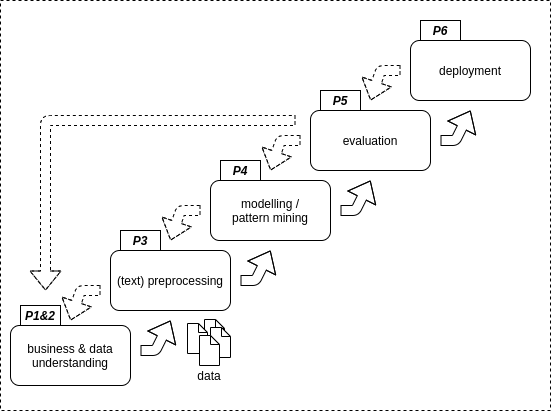
\includegraphics[width=0.9\linewidth]{media/nlp-workflow.png}
    \caption{CRISP-DM 1.0 Modell (eigene, abgeänderte Darstellung)}
    \label{fig:nlp_workflow}
\end{figure}

\lipsum[1]

\subsection{Maschinelles Lernen}
\label{sec:maschinelleslernen}

\lipsum[2]

\subsection{SpaCy Architektur}
\label{sec:spacyarchitektur}

\lipsum[1]

\section{Text Vorverarbeitung}
\label{subsec:textvorverarbeitung}

\lipsum[3]

\subsection{Tokenisierung}
\label{subsec:tokenisierung}

\lipsum[3]

\subsection{Stoppwörter entfernen}
\label{subsec:stoppwörter}

\lipsum[3]

\subsection{Wortart / Part of Speech}
\label{subsec:pos}

\lipsum[3]

\begin{figure}[!ht]
    \centering
    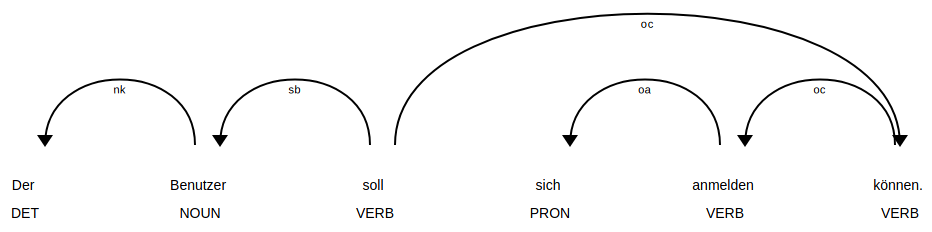
\includegraphics[width=\linewidth]{media/displaCy.png}
    \caption{POS-Muster und Abhängigkeit der Wörter}
    \label{fig:spacy_dependency}
\end{figure}

\lipsum[3]

\subsection{Lemmatisierung}
\label{subsec:lemmatisierung}

\lipsum[3]

\section{Merkmalextraktion}
\label{sec:merkmalextraktion}

\lipsum[3]

\section{Themenmodellierung mit LDA}
\label{subsec:themenmodellierung}

\lipsum[3]

\begin{figure}[!ht]
    \centering
    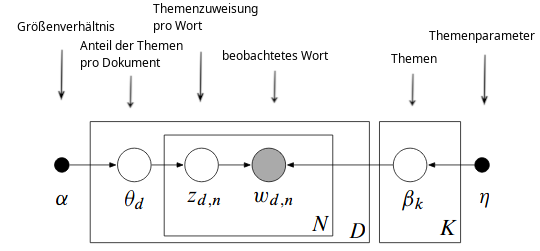
\includegraphics[width=0.9\linewidth]{media/LDA_selbst.png}
    \caption[LDA als grafisches Model mit eigenen Beschriftungen]{LDA als grafisches Modell}
    \label{fig:lda}
\end{figure}

\lipsum[3]

\section{Evaluierung}
\label{sec:evaluierng}

\lipsum[3]

\subsection{Konfusionsmatrix}
\label{sec:konfusionsmatrix}

\lipsum[3]

\begin{table}[!ht]
    \centering
    \begin{adjustbox}{width=0.65\columnwidth, center}
    \resizebox{\textwidth}{!}{
        \begin{tabular}{cccc}
         &  & \multicolumn{2}{c}{\textit{Vorhergesagt}} \\ \cline{3-4} 
         & \multicolumn{1}{c|}{} & \multicolumn{1}{c|}{Positiv} & \multicolumn{1}{c|}{Negativ} \\ \cline{2-4} 
        \multicolumn{1}{c|}{\multirow{2}{*}{\textit{Tatsächlich}}} & \multicolumn{1}{c|}{True} & \multicolumn{1}{c|}{TP} & \multicolumn{1}{c|}{FN} \\ \cline{2-4} 
        \multicolumn{1}{c|}{} & \multicolumn{1}{c|}{False} & \multicolumn{1}{c|}{FP} & \multicolumn{1}{c|}{TN} \\ \cline{2-4}
        \end{tabular}
    }
    \end{adjustbox}
    \caption{Konfusionsmatrix}
    \label{tab:confusionmatrix}
\end{table}

\lipsum[3]

\begin{eqnarray}
    F1 = 2\cdot \frac{precision\cdot recall}{precision+ recall}
\end{eqnarray}
